%%%%%%%%%%%%%%%%%%%%%%%%%%%%%%%%%%%%%%%%%
% University Assignment Title Page 
% LaTeX Template
% Version 1.0 (27/12/12)
%
% This template has been downloaded from:
% http://www.LaTeXTemplates.com
%
% Original author:
% WikiBooks (http://en.wikibooks.org/wiki/LaTeX/Title_Creation)
%
% License:
% CC BY-NC-SA 3.0 (http://creativecommons.org/licenses/by-nc-sa/3.0/)
% 
% Instructions for using this template:
% This title page is capable of being compiled as is. This is not useful for 
% including it in another document. To do this, you have two options: 
%
% 1) Copy/paste everything between \begin{document} and \end{document} 
% starting at \begin{titlepage} and paste this into another LaTeX file where you 
% want your title page.
% OR
% 2) Remove everything outside the \begin{titlepage} and \end{titlepage} and 
% move this file to the same directory as the LaTeX file you wish to add it to. 
% Then add \input{./title_page_1.tex} to your LaTeX file where you want your
% title page.
%
%%%%%%%%%%%%%%%%%%%%%%%%%%%%%%%%%%%%%%%%%
%\title{Title page with logo}
%----------------------------------------------------------------------------------------
%	PACKAGES AND OTHER DOCUMENT CONFIGURATIONS
%----------------------------------------------------------------------------------------

\documentclass[12pt]{article}
\usepackage[english]{babel}
\usepackage[utf8x]{inputenc}
\usepackage{amsmath}
\usepackage{graphicx}
\usepackage[colorinlistoftodos]{todonotes}
\DeclareMathOperator*{\argmax}{arg\,max} 
\begin{document}

\begin{titlepage}

\newcommand{\HRule}{\rule{\linewidth}{0.5mm}} % Defines a new command for the horizontal lines, change thickness here

\center % Center everything on the page
 
%----------------------------------------------------------------------------------------
%	HEADING SECTIONS
%----------------------------------------------------------------------------------------

\textsc{\LARGE Report}\\[1.2cm] % Name of your university/college
\textsc{\Large Models of Higher Brain Functions}\\[0.3cm] % Major heading such as course name
\textsc{\large Programming Project}\\[0.5cm] % Minor heading such as course title

%----------------------------------------------------------------------------------------
%	TITLE SECTION
%----------------------------------------------------------------------------------------

\HRule \\[0.4cm]
{ \huge \bfseries Reinforcement learning model of spatial navigation}\\[0.4cm] % Title of your document
\HRule \\[1.5cm]
 
%----------------------------------------------------------------------------------------
%	AUTHOR SECTION
%----------------------------------------------------------------------------------------

\begin{minipage}{0.4\textwidth}
\begin{flushleft} \large
\emph{Authors:}\\
Sören Becker, Jan Bölts % Your name
\end{flushleft}
\end{minipage}
~
\begin{minipage}{0.4\textwidth}
\begin{flushright} \large
\emph{Supervisor:} \\
David \textsc{Higgins} % Supervisor's Name
\end{flushright}
\end{minipage}\\[1cm]

%----------------------------------------------------------------------------------------
%	DATE SECTION
%----------------------------------------------------------------------------------------

{\large \today}\\[2cm] % Date, change the \today to a set date if you want to be precise

%----------------------------------------------------------------------------------------
%	LOGO SECTION
%----------------------------------------------------------------------------------------


\includegraphics[scale=.5]{figures/logo.jpg}\\[1cm] % Include a department/university logo - this will require the graphicx package
 
%----------------------------------------------------------------------------------------

\vfill % Fill the rest of the page with whitespace

\end{titlepage}

\section{Introduction}
\label{sec:intro}
This report describes a computational approach of learning an optimal strategy for a navigation task in a previously unknown environment. This kind of learning objective is a classical problem in the domain of reinforcement learning. 

Generally, in reinforcement learning an agent improves its performance on a given task by iteratively applying different actions, observing their consequences and learning from this experience. In the beginning of the learning process, the agent is completely ignorant to the task and has to explore its options of interaction with the environment in order to reach a predefined goal. Having reached the goal, a positive reinforcer is disposed, which indicates that the sequence of chosen actions led to the solution. The agent can use the reinforcer to update its preferences on action choices in order to improve its performance in the future. 

Since the agent is ignorant to the task at the beginning, meaning that no prior well-grounded preferences exist, it needs to perform random actions until it reaches the goal. On the second attempt to the task, the agent could in principle repeat the previous sequence of actions as this already led to the goal on the previous attempt. However, there is in general no justification to believe that the previous sequence of actions is optimal in the sense that it represents the shortest or least costly solution. The agent can therefore not simply exploit its experience. Hence, a major challenge in reinforcement learning, which is known as the exploration-exploitation-dilemma is to find a good trade-off between active exploration of possible actions and exploitation of already gathered experience. One way of dealing with this dilemma is to let the agent act according to some kind of policy which allows both random exploration of actions and action choices based upon experience. The ratio of random choices can then be gradually lowered with the increasing number of repetitions of the task to increase the reliance on experience. This broad concept of reinforcement learning is inspired by the introductions given in Sutton and Barto, 2012, and Watson, 1989, and describes the general learning framework that this report is concerned with. 

In particular, in the experiment investigated in this report, the environment consists of a T-shaped maze and the agent's task is similar to the stick-throwing game often played with dogs. Specifically, the agent starts at the lower end of the maze and has to learn by interacting with the environment to first go to the pick-up area located at the right end of the horizontal arm of the maze before going to the target area located at the left end of the horizontal arm. Difficulties of this task include that the agent has to learn the shape of the maze and that it needs to go to the pickup area before going to the target area as only then a reward is disposed. We investigate the agent's learning ability under a number of different parameter settings which effictively impact the number of possible action choices, the trade-off between exploration and exploitation, and the effect of memory-decay of an action's consequences.

The report is organized in the following way: an informal description of reinforcement learning and the investigated task is given in this section, a detailed, formal description of the simulated experiment and the employed methods is provided in section 2. In section 3 we describe the results of different parameter settings on the agent's learning ability which are discussed and explained in section 4.


\section{Methods}
\label{sec:methods}
This section provides a formal description of the simulated environment and task intended to be solved, the agent's internal representations, and lastly the applied learning algorithm. 

\subsection{Environment \& Task:}
The environment for the simulation is a T-shaped maze. The horizontal arm of the maze has a length of 110 cm and the vertical arm has a length of 50 cm while both have a width of 10 cm. The pickup and reward area cover the endmost 20 cm on both sides of the horizontal arm respectively. The geometry of the environment is depicted in Figure \ref{fig:geo}. In each simulation, the agent starts at the lower end of the maze and has to move into the pickup area before proceeding to the reward area to successfully finish one trial. If the agent attempts to step out of the boundaries of the maze, it receives a negative reward of -1 but remains at its current position, i.e., the illegal step out of the maze is not carried out. Furthermore, the agent receives a positive reward of +20 if it steps into the reward area after visiting the pickup area which automatically terminates a trial as this represents a completion of the task. No other rewards are disposed and in particular no reward is disposed at the target area if the pickup area has not been visited yet. 

\begin{figure}[h]
\centering
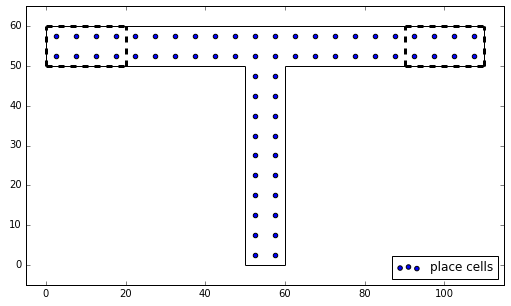
\includegraphics[width=1\textwidth]{figures/geometry.png}
\caption{\label{fig:geo} The geometry of the environment. The wall of the T-shaped maze are indicated by black lines, the target areas by dotted lines and the place cell centers by blue dots.}
\end{figure}

\subsection{Agent}
The agent's representation of the environment consists of two populations each containing n = 64 neurons. Specifically, the maze is divided by a regular grid into 64 fields of equal size and each neuron's activity is modeled as a location-dependent radial basis function that is placed at the center of one of these fields. One of the two populations is only active while the agent has not yet visited the pickup area whereas the other population is only active while the agent has already visited the pickup area. Formally, the activation of a neuron is given by 
\begin{align}
r_{j, \beta}(s) = \delta_{\alpha \beta} \exp(-\frac{(x_j - x)² + (y_j - y)²}{2\sigma²})
\end{align}
where $j=1,...,64$ indexes a neuron in population $\beta = \{0,1\}$. Variable $\alpha = \{0,1\}$ expresses whether the pickup area has been visited and $\delta_{\alpha, \beta}$ denotes Kronecker's delta, which ensures that only one of the two population is active. The placement of the radial basis function on the maze is given by ($x_j, y_j$) and its width is set to $\sigma = 5$ throughout all simulations. Each radial basis function is thus effectively a function of the triplet $s=(x, y, \alpha)$, i.e., the position and a boolean variable indicating a visit of the pickup area. This arangement of a spatial representation resembles place cells found in the hippocampus of rats and we therefore adopt the term place cells henceforth. The activations of the place cells are linearly combined to obtain a set of output neurons $Q_1,...,Q_m$ such that
\begin{align}
Q_a(s) = \sum_{j, \beta}w_{a j \alpha} r_{j \beta}(s) 
\end{align}
The output neurons are indexed by $a = 1,...,m$, where $m$ is the number of possible movements of the agent. The activation of the output neurons represent the action preferences for each state $s=(x,y,\alpha)$ and are optimized by adapting the weights $w_{aj\alpha}$ according to the learning algorithm. The agent moves through the maze by selecting a direction $\theta_i$ from a set $\{\theta_1 = 0,...,\theta_m = \frac{m-1}{0.5 \cdot m} \cdot \pi\}$ and updating its position according to
\begin{align}
x \leftarrow x + s \cdot \sin(\theta_i)\\
y \leftarrow y + s \cdot \cos(\theta_i)
\end{align}
For each step of the agent, the stepsize $s$ is drawn as a random sample from a normal distribution with $\mu = 3$ and $\sigma = 1.5$. We investigated the agent's behavior for $m = \{4, 8, 16\}$ directions which always covered $2\pi$ with a regular angular spacing. 

\subsection{Learning algorithm}
The weights $w_{aj\alpha}$ were optimized accoring to the SARSA algorithm in conjunction with an $\epsilon$-greedy policy for direction choices. The $\epsilon$-greedy policy allows the agent at each step with probability $\epsilon$ to select a random direction and forces it with probability $1-\epsilon$ to select the direction whose corresponding output neuron exhibits the highest activity:
\begin{align}
\theta = \begin{cases}
\mathcal{U}\{0, \theta_m\} &\text{with prob = $\epsilon$}\\
\theta_{a^*}\text{ for } a^* = \argmax\limits_a Q_a(s) &\text{with prob = $1 - \epsilon$}
\end{cases}
\end{align}
Policy parameter $\epsilon$ captures the trade-off between exploration and exploitation and decays exponentially at each step according to 
\begin{align}
\epsilon_{t+1} \leftarrow \epsilon_t \cdot 0.1^{\frac{1}{0.7 \cdot T}}
\end{align}
where $T$ is the number of simulated trials until $\epsilon$



\section{Results}
\label{sec:results}
\begin{figure}[h]
\centering
\includegraphics[width=0.7\textwidth]{figures/learning_curvet400r10.png}
\caption{\label{fig:sim1}Learning curve averaged over 10 runs. 400 trials, 4 actions, $\gamma=0.95$, $\lambda=0.4$, $\epsilon$ decaying exponentially to 0.1.}
\end{figure}
Figure \ref{fig:sim1} shows the learning curve of a simulation of 10 rats (runs) for 400 trials with escape latency averaged over all animals. A learning effect can be observed already after few trials. After about 100 trials the rat seems to have found the optimal path, i.e., learning has converged. It then needs about 60 steps to obtain the reward at the target. 
\begin{figure}[h]
\centering
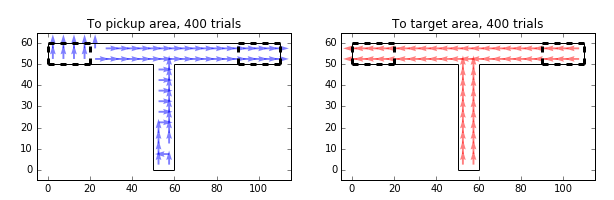
\includegraphics[width=1\textwidth]{figures/navigation_map.png}
\caption{\label{fig:nav}This is a figure caption.}
\end{figure}

A visualization of the animals behavior is shown in Figure \ref{fig:nav}. We plotted a vector field showing the directions of preferred actions inferred from the maximal Q-value for the center of every place field. The two subplots refer to the two subtask of finding the pickup area and subsequently finding the target area. For the first subtask, i.e., on the way to the pickup area, almost all preferred actions point towards to pickup area. Once that is reached, the preference changes and the majority of vectors point towards the target area. 

\begin{figure}[h]
\centering
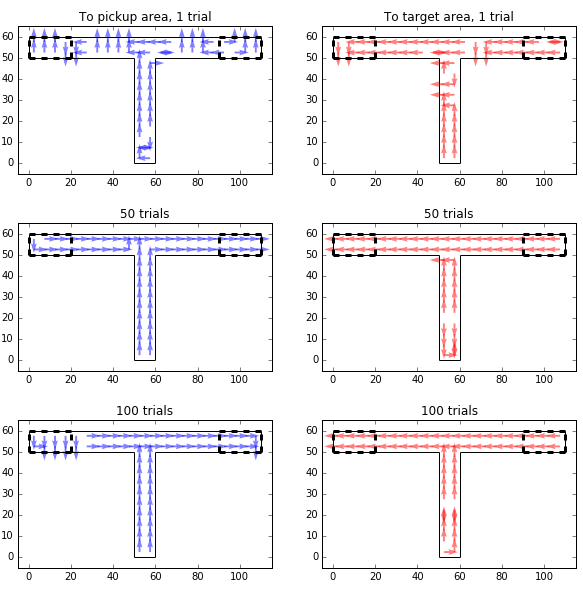
\includegraphics[width=1\textwidth]{figures/navigation_map_trials.png}
\caption{\label{fig:nav_trials}Navigation maps after 1, 5 and 100 trials, respectively (rows) and on the way to pickup and to target, respectively (columns).}
\end{figure}

Figure \ref{fig:nav_trials} shows the development of the navigation maps over trials. The rows of subplots corresponds to the navigation map after 1 trial, 50 trials and 100 trials, respectively. One can observe a goal directed change already after 1 trial, e.g., on the way to the target. However, clearly goal directed behavior for all locations develops only after 100 trials. 

The decay of memories seems to be a crucial point in the learning process of the agent. Figure \ref{fig:lc_lam} shows the learning curves for different values of the memory decay parameter $\lambda$. Note the different scales on the y-axis and the number of trials on the x-axis after which learning converges. Interestingly, learning seems to be most effective for a moderate decay around $\lambda=0.5$. For other values learning occurs later ($\lambda=0.2$) or not at all ($\lambda=0.9$). 

\begin{figure}[h]
\centering
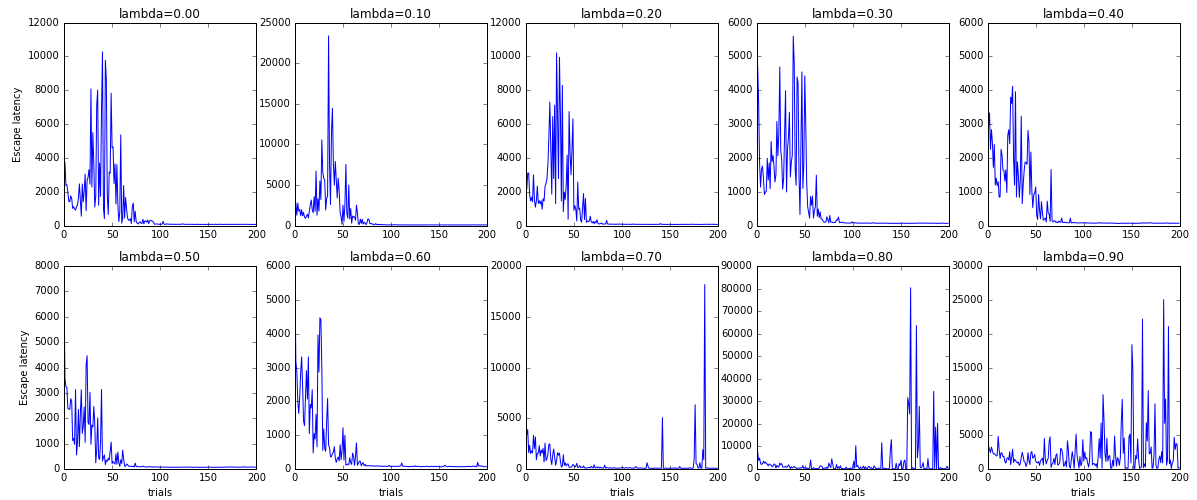
\includegraphics[width=1\textwidth]{figures/learning_curve_lambda.png}
\caption{\label{fig:lc_lam} Learning curves for difference values of memory decay parameter $\lambda$. 200 trials, averaged over 5 runs, $\gamma=0.95$.}
\end{figure}

In order to solve the exploration/exploitation dilemma it is useful to use a time-varying exploration/exploitation parameter $\epsilon$. Figure \ref{fig:eps} shows the time course of the $\epsilon$ parameter. It is close to 1 in the beginning and then decays exponentially to 0.1 within $70\%$ of the given number of trials. 

\begin{figure}[h]
\centering
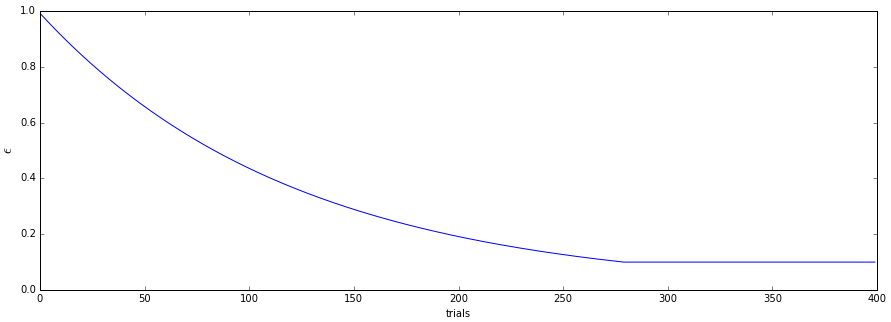
\includegraphics[width=.8\textwidth]{figures/epsilon_timecourse.png}
\caption{\label{fig:eps}The time course of the $\epsilon$ parameter over 400 trials.}
\end{figure}

Finally, the effect of varying number of possible actions on the learning process was investigated. Figure \ref{fig:lc_act} shows the learning curves for different numbers of possible actions. The more actions the agent can choose from, the longer it needs to learn the task. Interestingly, the escape latency decreases first and then increases again for both, the case 8 and the case of 16 possible actions. 

\begin{figure}[h]
\centering
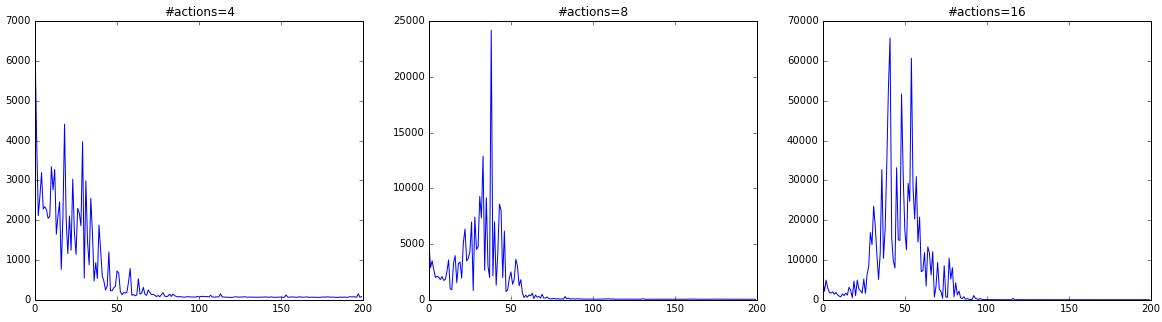
\includegraphics[width=1\textwidth]{figures/learning_curve_actions.png}
\caption{\label{fig:lc_act} Learning curves for different numbers of actions. 200 trials, averaged over 5 runs, $\lambda=0.6$.}
\end{figure}

\section{Discussion}
This section will discuss and explain the results that were presented in the previous sections. It will comment on the question that were given in the project description. 

The initial simulation consisted in 10 runs with 400 trials each and calculated the escape latencies over trials, averaged over all runs. This was in order to quantify how long the takes the rat learn the task. We state that the rat has learned the task if there is no more, or very little, variation in the escape latencies and if the escape latency is close to the theoretical optimum. From the results given above we can see that this is the case after about 100 trials. However, this result depends on how fast the rat switches from exploration to exploitation, i.e., if we were to reduce the number of trials and increase the rate with which $\epsilon$ decays to 0.1, we rat might be able to learn even faster. This comes with the risk that it might not find the optimal path because it does not exlpore long enough. Figure \ref{fig:lc_trials} shows the learning curves after different number of trials, averaged over 5 runs. Only $70\%$ of the given number of trials is used for learning, i.e., after that $\epsilon=0.1$. One can observe that under these circumstances, the rat is able to learn the task within 30 trials. 

\begin{figure}[h]
\centering
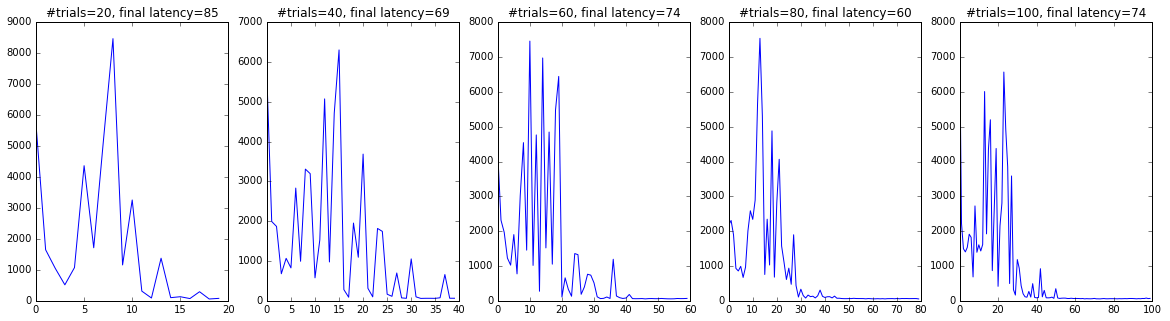
\includegraphics[width=1\textwidth]{figures/learning_curve_trials.png}
\caption{\label{fig:lc_trials} Learning curves for different numbers of trials. Averaged over 5 runs, $\lambda=0.5$, $70\%$ of trials for learning.}
\end{figure}

We presented a visualization of the agent's behavior by plotting a vector field of preferred movement direction for every place cell center position in Figure \ref{fig:nav} and \ref{fig:nav_trials}. The results show that for the navigation map of the subtask of finding the way to the target, many arrows point toward the target area in the upper left arm already after the first trial. For the navigation map of the subtask of finding the pickup area this is not the case. This may be due to the fact the information of the reward needs more trials to spread to earlier stages of the task. Consequently, after 50 trials, both navigation maps show clearly goal directed preferred movement directions, i.e., for both navigation maps the preferred movement direction in the vertical arm is upwards, then, before the pickup area is reached (blue arrows) the preferred movement direction in the horizontal arm is to the right and after the pickup area was reached it changes to the left (red arrows). 


\section{Acknowledgements}
We would like to thank Steffen Puhlmann for helping us to debug our code. And finally, many thanks to David Higgins for supervising this project. 
\end{document}